\documentclass{article}
\usepackage[margin=1in]{geometry}
\usepackage{fancyvrb}
\usepackage{multicol}
\usepackage{hyperref}
\usepackage{amsmath}
\usepackage{amsfonts}

\usepackage[listings]{tcolorbox}

\definecolor{codegreen}{rgb}{0,0.6,0}
\definecolor{codegray}{rgb}{0.5,0.5,0.5}
\definecolor{codepurple}{rgb}{0.58,0,0.82}
\definecolor{backcolour}{rgb}{0.95,0.95,0.92}

\lstdefinestyle{mystyle}{
    language=Python,
    backgroundcolor=\color{backcolour},   
    commentstyle=\color{codegreen},
    keywordstyle=\color{magenta},
    numberstyle=\tiny\color{codegray},
    stringstyle=\color{codepurple},
    basicstyle=\ttfamily\footnotesize,
    breakatwhitespace=false,         
    breaklines=true,                 
    captionpos=b,                    
    keepspaces=true,                 
    numbers=left,                    
    numbersep=5pt,                  
    showspaces=false,                
    showstringspaces=false,
    showtabs=false,                  
    tabsize=2,
    escapechar=|,
    frame=single
}

\lstset{style=mystyle}

%\usepackage[T1]{fontenc}
\usepackage{tikz}
\usetikzlibrary{arrows.meta,
                calc, chains,
                decorations.pathreplacing,
                calligraphy,
                positioning,
                quotes,
                shapes}
                
\newcommand{\showfig}[2]{
\noindent\includegraphics[width=\textwidth]{#1}
\centerline{#1}
}
\newcommand{\bi}{\begin{itemize}}
\newcommand{\li}{\item}
\newcommand{\ei}{\end{itemize}}

\title{Linked List Bignums}
\author{CSCI 112, Lab 4}
\date{}

\begin{document}
\sloppy

\maketitle

\begin{description} 
\item[File names:]  Names of files, functions, and variables, 
when specified,
must be EXACTLY as specified.  This includes simple mistakes such
as capitalization.

\item[Individual work:]  All work must be your own.  Do not share
code with anyone other than the instructor and teaching assistants.
This includes looking over shoulders at screens with the code open.
You may discuss ideas, algorithms, approaches, {\em etc.} with
other students but NEVER actual code.  Do not use code
written by anyone else, in the class or from the internet.

\item[Documentation:] Each file should begin with a docstring
that includes your name, the class number and name, the lab
number, and  
a short description of the lab, as well as documentation pertinent
to that particular file.

\item[Addition and subtraction standard algorithm:]  You should be
familiar with the standard algorithms for addition and subtraction,
at least in base 10.  If you are not familiar with other number bases,
review them quickly here: \url{https://www.mathsisfun.com/numbers/bases.html}.

The standard subtraction and addition algorithms work fine in any
base.  You just have to remember that if you are in base 16, say,
and you ``borrow one'' from the next column, you are borrowing 16,
not 10.  Likewise, you ``carry one'' to the next column when you
get 16 or more, not 10.  Here are some worked examples to get
the hang of things:

Base 10 examples:\hfill
\begin{tabular}{rrrrr}
  &3 &9 &1 &5\\
$+$ &1 &2 &4 &5\\
\hline
  &5 &1 &6 &0\\
\end{tabular}\hfill
\begin{tabular}{rrrrr}
  &3 &9 &1 &5\\
$-$ &1 &2 &4 &5\\
\hline
  &2 &6 &7 &0\\
\end{tabular}

Base 8 examples:\hfill
\begin{tabular}{rrrrrr}
  &  &7 &5 &1 &3\\
$+$ &  &2 &3 &3 &5\\
\hline
  &1 &2 &0 &5 &0\\
\end{tabular}\hfill
\begin{tabular}{rrrrr}
  &7 &5 &1 &3\\
$-$ &2 &3 &3 &5\\
\hline
  &5 &1 &5 &6\\
\end{tabular}

Base 16 examples:\hfill
\begin{tabular}{rrrrr}
  &  &15 &4 &11\\
$+$ &  &4 &13 &13\\
\hline
  &1 &4 &2 &8\\
\end{tabular}\hfill
\begin{tabular}{rrrr}
  &15 &4 &11\\
$-$ &4 &13 &13\\
\hline
  &10 &6 &14\\
\end{tabular}

If you want more examples, just run my program {\tt arithmetic.py}
and paste the output into a new project on \url{https://www.overleaf.com}.

You can get easy base 8 and base 16 examples from python (remember that
in base 16 the digits 10 to 15 are: {\tt a, b, c, d, e, f}):
\begin{lstlisting}
>>> hex(0xaaa + 0x123)
'0xbcd'
>>> oct(0o666 + 0o123)
'0o1011'
\end{lstlisting}

\item[Bignums:]  Python has bignums (arbitrarily high integers) built in.  For example, Python
has no problem computing:
\begin{lstlisting}
>>> 1234567890987654321 * 1234567890987654321
1524157877457704723228166437789971041
\end{lstlisting}
Even though computers only natively support either 32 bit integers, or 64
bit integers.  Hence, the maximum integers supported in most programming
languages are either $2^{32} = 4.294.967.296$ or  $2^{64} = 18.446.744.073.709.551.616$.
Integers larger than this are supported in software.

When Python encounters integers that are too big for the 32 or 64 bit
registers, it automatically converts them to bignums.  

In this lab we will build a Bignum class of our own that supports arbitrarily large integers
using linked lists.  Each cell in the linked list will hold a single position in
the base.  For example, if we choose base 10 for our bignums, each
cell in the linked list will hold a Python integer from 0 to 9.  If we choose
base 16 for our bignums, each cell in the linked list will hold a 
Python integer between 0 and 15.  If we choose 10,000 for our base,
each cell in the linked list will hold a Python integer between 0 and 9,999.

Here, for example, is a figure of what the number \lstinline{0o374} in base 8
looks like:

\begin{center}
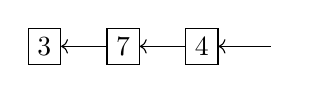
\begin{tikzpicture}
\tikzset{
  block/.style={draw, rectangle}
  }
\node[block] (A) {3};
\node[block,right of=A] (B) {7};
\node[block,right of=B] (C) {4};
\node[right of=C] (D) {};
\draw[->] (D) -- (C);
\draw[->] (C) -- (B);
\draw[->] (B) -- (A);
\end{tikzpicture}
\end{center}

Note that the smallest digit will be at the head of the list.  This will make arithmetic
much easier.

Make your Bignum class general, so it will support any base.

\item[Signs:]  Positive and negative numbers will be represented by
a separate field in the class called \lstinline{Bignum.sign}, with the value
of either plus or minus one.

\item[Initializing and extracting Python ints:]  To make testing easy, Bignums will be initialized
by Python integers.  The initializing integer can be any size, of course,
using Python's native integers.  You will convert this to your linked list
representation of Bignums.

Also to make testing easy, include a \lstinline{Bignum.int} method that
converts your bignum into a Python int.  This will support easy testing
expressions such as:
\begin{lstlisting}
n = 2**100_000
self.assertEqual(n, Bignum(n).int())
\end{lstlisting}

\item[Addition and subtraction:]  Once you've got your Bignum class
working, 
implement the standard algorithms for addition and subtraction, as illustrated
above, to support the \lstinline{__add__} and \lstinline{__sub__} methods
for your Bignums.  

You will have to do a little sign checking at the beginning.  For example,
to subtract a negative number from a positive number, just convert the negative
to a positive and then add.  Or, for another example, 
to subtract a larger number, $a$, from a smaller number, $b$, use the formula:
\[
b - a = -(a = b)
\]
So you will alwasy be subtracting the smaller from the larger.   There are a few
other cases for you to work out: each operand can be positive or negative,
and either one could be the larger.  There should be eight cases in all, then, right?

\item[Leading zeros:]  Some operatrions may result in leading zeros, for example,
$12345 - 12300$ in base 10.  Your Bignum class should clean up any result
by removing these unecessary zeros.


\item[Multiplication:]
The standard algorithm for multiplication is somewhat complex to implement
using our representation.  Fortunately, there is a way to compute the product
in $O(\log n)$ time just using addition and subtraction:
\[
ab = \left\{\begin{array}{ll}
0    &  \mbox{if $b=0$}\\
a + a(b-1)  & \mbox{if $b$ is odd}\\
2(a(b/2)) &\mbox{otherwise}
\end{array}\right.
\]
You will also have to implement division by 2.  This should be easy.  Just think
carefully about how you do it using the standard long division algorithm, and
remember when you ``carry'' or ``borrow'' 1, you are carrying or borrowing
the base amount, not 10.

Implement this strategy to support the \lstinline{__mul__} method for your
bignums.  Again, make sure you handle the signs.  It will be slightly quicker if
you alwasy choose the smaller number for the recursion, right?

\item[Calculator:] Use your infix calculator from the previous lab to
make a Bignum calculator!

\item[Timing:]  Run some experiments to see how the timing of your
Bignums changes with the size of the base.  Note that Python will
not use native integers if the size of the integer is greater 
than the size of a native integer.  Since your calculations can result
in numbers in the cells up to base$^2$, your base should probably
not exceed $2^{16}$ for 32 bit computers, or $2^{32}$ for 64 bit
computers.  (Why?)

Once you find the best base for your implementation, compare
times on your implementation with those for native Python bignums.
How much slower are you?  Do you think it makes a big-O difference,
or not?  Why?

Write up your experiments and conclustions in a short document.

\item[Optional:]  Division!  Exponentiation!  Implement \lstinline{gcd} and search for
large primes!
    
\end{description}



\end{document}
